\documentclass[12pt,a4paper]{article}
\usepackage[UTF8]{ctex}
\usepackage{graphicx}
\usepackage{geometry}
\usepackage{ulem}
\usepackage{enumitem}
\usepackage{titlesec}
\usepackage{multicol}
\usepackage[export]{adjustbox}
\usepackage{amsmath}  % 推荐用于更好的数学排版
\usepackage[utf8]{inputenc}
\usepackage{CJKutf8}
\usepackage{fancyhdr}
\usepackage{lastpage}
\usepackage{ulem}
\usepackage{tabularx}
\usepackage{lastpage}
\usepackage{float}
\usepackage{subcaption}
\usepackage{multicol}
\usepackage{multirow}
% 页眉页脚设置
\pagestyle{fancy}
\fancyhf{} % 清除所有页眉页脚
% 设置页眉内容
%-==========1. 填写从第二页开始 每页第一行的信息==========-
\fancyhead[C]{
    \footnotesize
    \makebox[4.5em][c]{实验名称：} \uline{\makebox[18em][c]{晶体管共射放大电路的设计、仿真与测试}} 
    \makebox[2.5em][c]{姓名：} \uline{\makebox[4em][c]{}} 
    \makebox[2.5em][c]{学号：} \uline{\makebox[5em][c]{}}
}%--------------------------------------------------------
\fancyfoot[C]{第 \thepage\ 页，共 \pageref{LastPage} 页}

% 取消页眉和页脚的下划线
\renewcommand{\headrulewidth}{0pt} % 页眉横线粗细设为0
\renewcommand{\footrulewidth}{0pt} % 页脚横线粗细设为0

% 调整页眉高度
\setlength{\headheight}{50pt}

% 设置plain样式（用于第一页）
\fancypagestyle{plain}{
    \fancyhf{} % 清除所有页眉页脚
    \renewcommand{\headrulewidth}{0pt} % 隐藏页眉横线
    \fancyfoot[C]{第 \thepage\ 页，共 \pageref{LastPage} 页} % 保留页脚
}
% 设置页面边距
\geometry{left=2.54cm,right=1.5cm,top=2.54cm,bottom=2.54cm}

% 设置正文字体大小为小四
\renewcommand{\normalsize}{\fontsize{12pt}{18pt}\selectfont}
% 设置章节格式
\titleformat{\section}{\fontsize{16pt}{24pt}\selectfont\bfseries}{\thesection}{1em}{} % 一级标题：三号
\titleformat{\subsection}{\fontsize{15pt}{22.5pt}\selectfont\bfseries}{\thesubsection}{1em}{} % 二级标题：小三

\begin{document}
\thispagestyle{plain}%第一页使用 plain 样式，而不是默认的 fancy 样式，第一页不再显示页眉
% 标题部分 - 两栏布局
\begin{multicols}{2}
    % 左栏：图片和实验报告标题
    % 左栏：使用空行创建前三行
    \noindent
    ~\\ % 第一行
    ~\\ % 第二行
    ~\\ % 第三行
    \hphantom{占位}% 使用空占位符
    \raisebox{-0.5\baselineskip}% 图片向下移动半行
    {
\includegraphics[width=1.85in,height=0.58in]{figure/ZJU.jpg}}
    \hspace{.5em}% 图片和标题之间的间距
    \raisebox{0pt}[\height][0pt]% 标题底部对齐
    {\textbf{\fontsize{26pt}{30pt}\selectfont 实验报告}}
    
    \columnbreak % 换到右栏
    
    % 右栏：个人信息
    % 右栏：个人信息 - 靠右对齐 
%-==========2. 填写个人信息==========-
    \begin{flushright}
        \makebox[3em][l]{专业：} \uline{\makebox[9em][c]{}} \\
        \makebox[3em][l]{姓名：} \uline{\makebox[9em][c]{}} \\
        \makebox[3em][l]{学号：} \uline{\makebox[9em][c]{}} \\
        \makebox[3em][l]{日期：} \uline{\makebox[9em][c]{2025年12月2日}} \\
        \makebox[3em][l]{地点：} \uline{\makebox[9em][c]{紫金港东四216}} \\
    \end{flushright}   
\end{multicols}
% 课程名称等信息（单栏）
%-==========3. 填写课程信息==========-
\noindent\small
\makebox[0.3\textwidth][l]{课程名称：\uline{电子电路设计实验I}}
\makebox[0.38\textwidth][l]{指导老师：\uline{施红军、叶险峰、邓靖靖}}
\makebox[0.1\textwidth][l]{成绩：\uline{\hspace{2cm}}}\\
\makebox[0.52\textwidth][l]{实验名称：\uline{晶体管共射放大电路的设计、仿真与测试}}
\makebox[0.22\textwidth][l]{实验类型：\uline{设计类实验}}
\makebox[0.2\textwidth][l]{同组学生姓名：\uline{}}
%-==========4. 正文开始==========-
\section*{一、实验目的}
学习晶体管放大电路的设计方法，掌握晶体管放大电路静态工作点的设置、测量与
调整方法，了解放大器的非线性失真，掌握放大器电压增益、输入电阻、输出电阻、幅频响应等基
本性能指标的测量方法，理解负反馈对放大电路性能的影响。
\section*{二、实验任务与要求}
1、设计一阻容耦合单级放大电路

已知条件：$V_{CC}=+9\mathrm{V}$，$R_L=5.1\mathrm{k}\Omega$，$V_i=10\mathrm{mV}$，$R_S=600\Omega$

性能指标要求：$f_L<50\mathrm{Hz}$，$|A_v|>15\mathrm{V/V}$，$R_i>3\mathrm{k}\Omega$

2、设计要求

（1）写出详细设计过程并进行验算

（2）用软件进行仿真

3、电路安装、调整与测量

自己编写调试步骤，自己设计数据记录表格

\section*{三、实验原理}
\subsection*{3.1 共射放大电路分析计算}
图 \ref{fig:1.1} 所示为分立电路中普遍采用的阻容耦合共射放大电路。它采用的是分压式电流负反馈
偏置电路。射极电阻 $R_{E1}$和$R_{E2}$ 都参与了直流电流负反馈，但只有 $R_{E1}$ 参与交流电流负反馈，因为旁
路电容 $C_E$ 交流时可认为短路。
\begin{figure}[H]
    \centering
    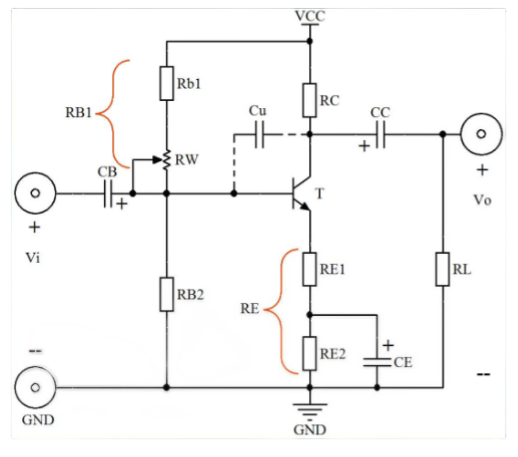
\includegraphics[width=0.4\textwidth, height=0.2\textheight]{figure/circuit.png}
    \caption{共射放大电路电路图}
    \label{fig:1.1}
\end{figure}

\subsection*{3.1.1 静态工作点分析计算}
静态工作点计算主要是确定晶体管的静态电流 $I_C$ 和集射静态压降 $V_{CE}$。$I_C$值可用来计算小信号
模型参数，进而计算放大电路的电压增益、输入电阻、输出电阻等主要性能指标，$V_{CE}$值用来判断晶
体管是否处于放大状态。

\begin{figure}[H]
    \centering
    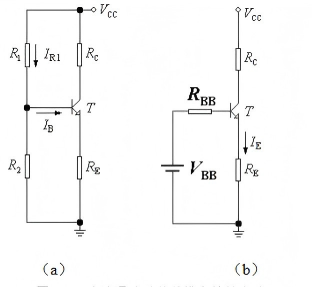
\includegraphics[width=0.4\textwidth, height=0.2\textheight]{figure/dc_circuit.png}
    \caption{直流通路及其戴维南等效电路图}
    \label{fig:1.2}
\end{figure}

戴维南等效电路中有
\[\left\{\begin{array}{l}
V_{B B}=V_{C C} \frac{R_{2}}{R_{1}+R_{2}} \\
R_{B B}=R_{1} \| R_{2}
\end{array}\right.\]

当晶体管处于放大状态时可得
\[
\left\{\begin{aligned}
I_{E} &=\frac{V_{BB}-V_{BE}}{R_{E}+\frac{R_{BB}}{(1+\beta)}} \\
I_{C} &=\frac{\beta}{1+\beta}I_{E}\approx I_{E} \\
V_{CE} &=V_{CC}-(R_{C}+R_{E})I_{C}
\end{aligned}\right.\]
\subsection*{3.1.2 交流性能指标计算}
三极管小信号模型参数
\[
\left\{\begin{array}{l}
g_{m}=\frac{I_{C}}{V_{T}} \\
r_{\pi}=\frac{\beta}{g_{m}} \\
r_{e}=\frac{\alpha}{g_{m}}
\end{array}\right.
\]
交流等效电路图如下
\begin{figure}[H]
    \centering
    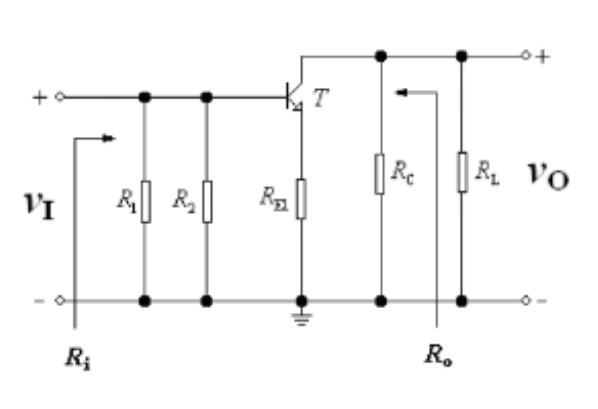
\includegraphics[width=0.4\textwidth, height=0.2\textheight]{figure/ac_circuit.png}
    \caption{交流通路电路图}
    \label{fig:1.3}
\end{figure}
此时有
电压增益
\begin{equation}
A_v = \frac{v_o}{v_i} \approx -\frac{\text{集电极总电阻}}{\text{发射极总电阻}} = \frac{-R'_C}{R'_E} = -\frac{R_C \parallel R_L}{r_e + R_{E1}}
\end{equation}
输入电阻
\begin{equation}
R_i=R_1 \parallel R_2 \parallel \left[(1+\beta)(r_e+R_{E1})\right]
\end{equation}
输出电阻
\begin{equation}
R_o \approx R_C
\end{equation}

通频带 $ BW = f_H - f_L $ \hspace{20pt} 

式中，$ f_H $ 为上限截止频率，主要受晶体管内部结电容及电路的分布电容限制；$ f_L $ 为下限截止频率，主要受射极旁路电容 $ C_E $ 及耦合电容 $ C_1 $、$ C_2 $ 影响。

要严格计算电容 $ C_1 $、$ C_2 $ 及 $ C_E $ 同时存在对放大器低频特性的影响较为复杂。工程上常用短路时间常数法进行简化计算。先求出每个电容单独存在时的转折频率 $ \omega_{c1} $、$ \omega_{c2} $、和 $ \omega_{c3} $，则这些电容同时存在时的下限截止频率为

\[f_L \approx \frac{1}{2\pi} \sqrt{\omega_{C1}^2 + \omega_{C2}^2 + \omega_{CE}^2} \hspace{20pt} \]
\subsection*{3.2 静态工作点与失真}

静态工作点过高或过低都容易产生非线性失真。若 Q 点过高，如图 \ref{fig:i_2.1.5} 所示的 Q1，稍大的输
入信号正半周将使晶体管进入饱和区，β 值明显减小，因而 ic 波形将出现顶部压缩、输出电压 $u_{ce}$
波形将在底部压缩，这称为饱和失真；若 Q 点太低，如图 \ref{fig:i_2.1.5} 所示的 Q2，稍大的输入信号负半周
将使晶体管进入截止区，因而 ic 波形将出现底部压缩、输出电压 $u_{ce}$ 波形将在顶部压缩，这称为截
止失真。

大信号工作时，为了得到最大不失真输出电压幅度，其静态工作点应设在交流负载线的中间位
置，如图 \ref{fig:i_2.1.6} 所示。但当输出信号幅度不是太大时，Q 点不一定要选在交流负载线的中点，而是可
根据其他要求来选择。例如，希望放大器耗电少、噪声低或输入阻抗高，Q 点可选得低一些；而当
希望放大器增益高时，就要求 Q 点适当高一些。

调整静态工作点的方法就是改变上偏置电阻 $R_1$ 的大小，即调节电位器的阻值，同时用万用表检
测集电极电阻 $R_C$ 两端压降，以判断 $V_{CE}$ 和 $I_C$ 是否为合适值。
\begin{figure}[H]
    \centering
    \begin{subfigure}[b]{0.32\textwidth}
        \centering
        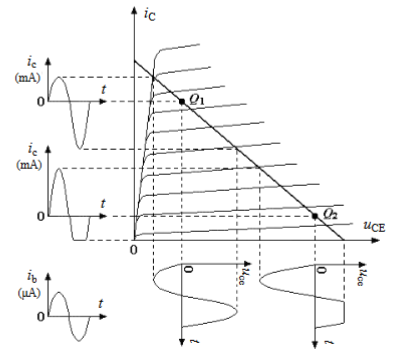
\includegraphics[width=\textwidth]{figure/i_2.1.5.png}
        \caption{静态工作点选取不当产生的非线性失真}
        \label{fig:i_2.1.5}
    \end{subfigure}
    \hfill

    \begin{subfigure}[b]{0.32\textwidth}
        \centering
        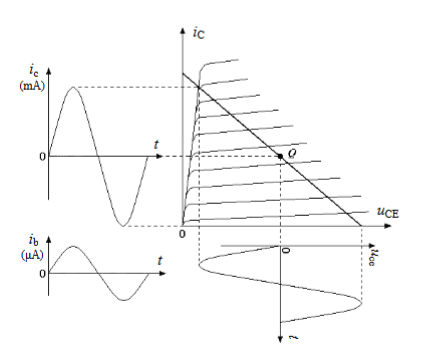
\includegraphics[width=\textwidth]{figure/i_2.1.6.png}
        \caption{为获得最大不失真输出电压的静态工作点选取}
        \label{fig:i_2.1.6}
    \end{subfigure}
    \hfill

    \caption{静态工作点与失真}
    \label{fig:distort_2}
\end{figure}
 
\section*{四、实验方案设计与参数计算}
\subsection*{4.1 实验方案总体设计}
已知条件  
\[ V_{cc} = 9V, R_L = 5.1k\Omega, V_i = 10mV, R_s = 600\Omega \]  

性能指标要求  
\[ |A_v| > 15V/V, R_l > 3k\Omega, f_L < 50Hz \]

计算过程如下：
\begin{figure}[H]
    \centering
    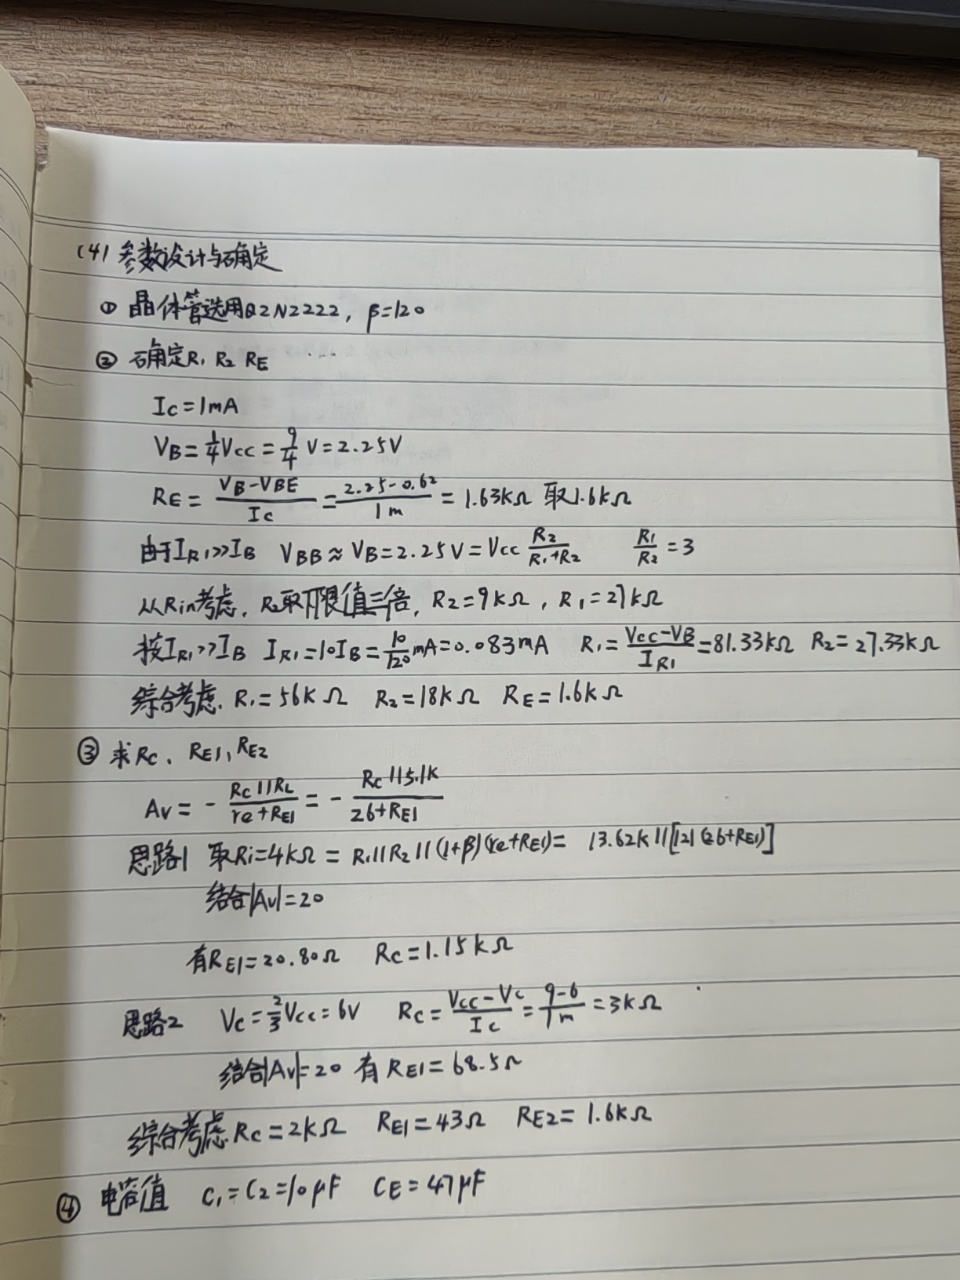
\includegraphics[width=0.4\textwidth, height=0.4\textheight]{figure/design_process.jpg}
    \caption{计算过程}
    \label{fig:design}
\end{figure}

最终元件值确定为 $R_1 = 56k\Omega, R_2 = 18k\Omega, R_C = 2k\Omega, R_{E1} = 43\Omega, R_{E2} = 1.6k\Omega, C_1 = 10\mu F, C_2 = 10\mu F, C_E = 47\mu F$

\subsection*{4.2 各功能电路设计验算}
设计参数：$V_{cc}=9V$, $R_L=5.1k\Omega$, $R_1=56k\Omega$, $R_2=18k\Omega$, $R_{E1}=43\Omega$, $R_{E2}=1.6k\Omega$, $R_C=2k\Omega$, $C_1=10\mu F$, $C_2=10\mu F$, $C_E=47\mu F$  

设计要求：$|A_{vo}|>15V/V$, $R_i>3k\Omega$, $f_L<50Hz$  

验算过程：
\begin{figure}[H]
    \centering
    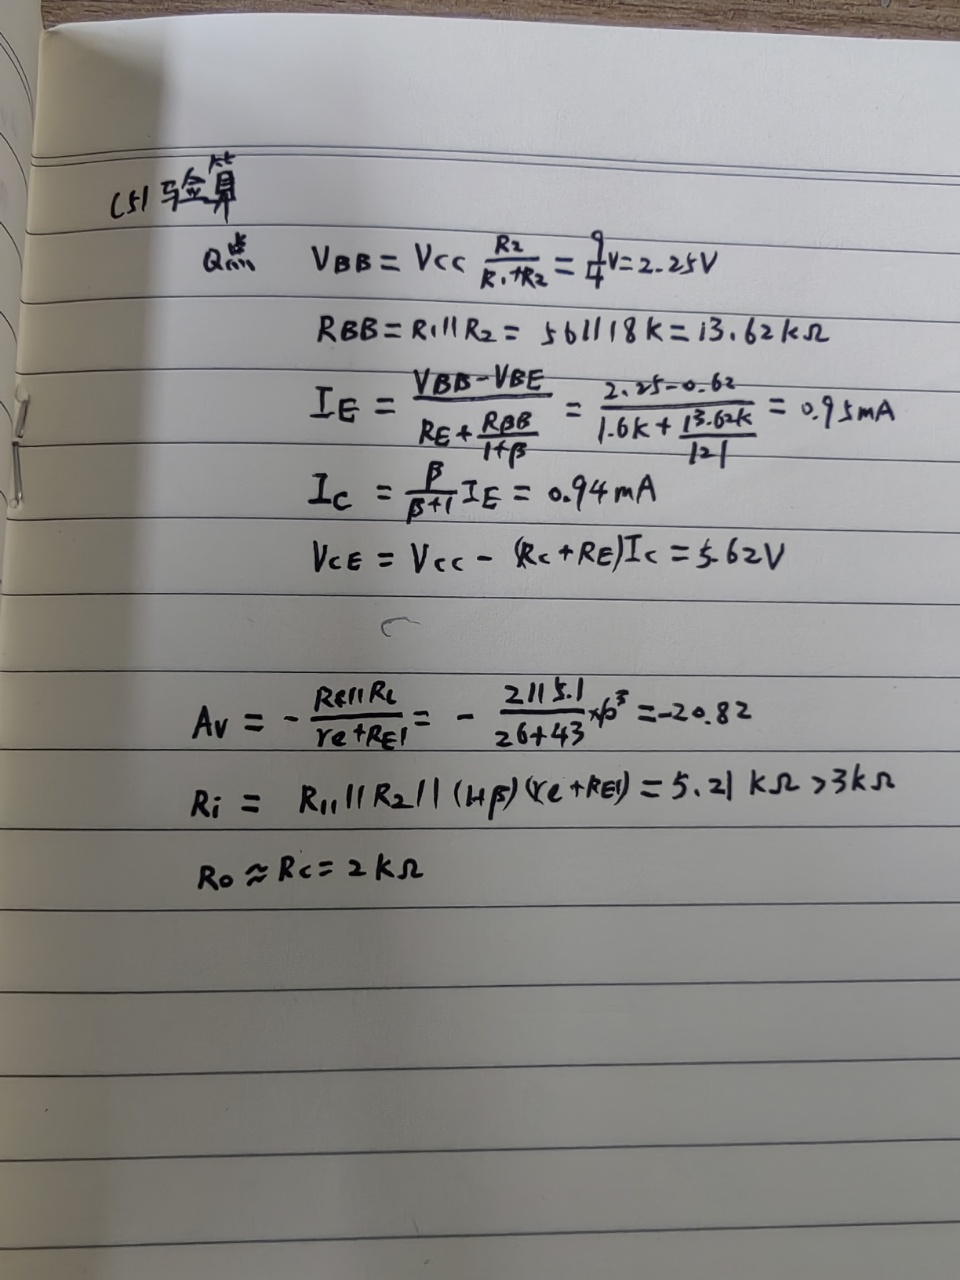
\includegraphics[width=0.4\textwidth, height=0.4\textheight]{figure/check_process.jpg}
    \caption{验算过程}
    \label{fig:check}
\end{figure}
设计时目标值：  
$|A_{vo}|>15V/V$, $R_i>3k\Omega$ 

验算结果：  
$|A_{vo}|=20.82V/V$, $R_i=5.21k\Omega$
满足设计要求。
\section*{五、实验仪器设备}
示波器，电源，电路板，信号发生器，导线，电阻、电容等电子元器件

\section*{六、实验步骤、调试过程、实验数据记录}
\subsection*{6.1 电路仿真}
\subsubsection*{6.1.1 静态工作点}
根据设计参数搭建电路并进行仿真，测得静态工作点数据如下表所示：
\begin{figure}[H]
    \centering
    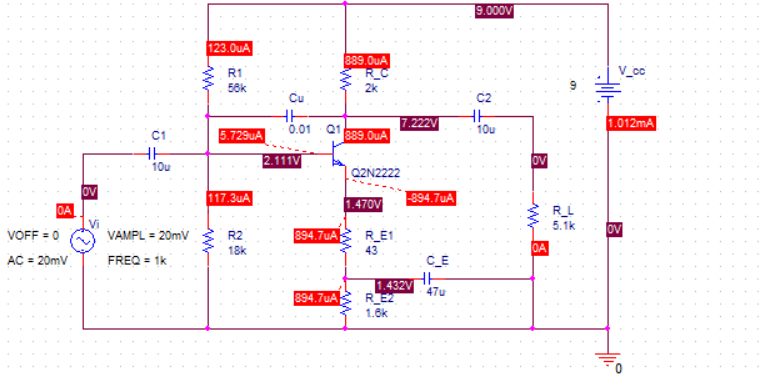
\includegraphics[width=0.4\textwidth, height=0.2\textheight]{figure/Q_sti.png}
    \caption{仿真电路图}
    \label{fig:1.4}
\end{figure}

根据仿真结果可以看到，静态工作点数据如下表所示：
\begin{table}[H]
    \centering
    \begin{tabular}{|c|c|c|c|c|c|c|}
    \hline
    $I_C$ ($\mu A$) & $V_{CE}$ (V) & $V_B$ (V) & $V_E$ (V) & $I_B$ ($\mu$A) & $I_{R1}$ ($\mu$A) & $I_{R2}$ ($\mu$A) \\
    \hline
    894.7 & 5.752 & 2.111 & 1.470 & 5.729 & 123.0 & 117.3 \\
    \hline
    \end{tabular}
    \caption{静态工作点测量数据}
    \label{tab:1.1}
\end{table}
\subsubsection*{6.1.2 电压增益与下限截止频率}
(1)进行交流分析。运行后在 Probe 窗口中，添加 V（RL：2）/V（Vi：+）作输出，显
示出频响特性，利用measure功能测得$|Av| = 19.68298,f_L=50.25532Hz ,f_H = 25.90266MHz$。
下限截止频率略大于预期的50kHz，表明设计电路的参数有瑕疵需要进一步优化。
\begin{figure}[H]
    \centering
    \begin{subfigure}[b]{0.32\textwidth}
        \centering
        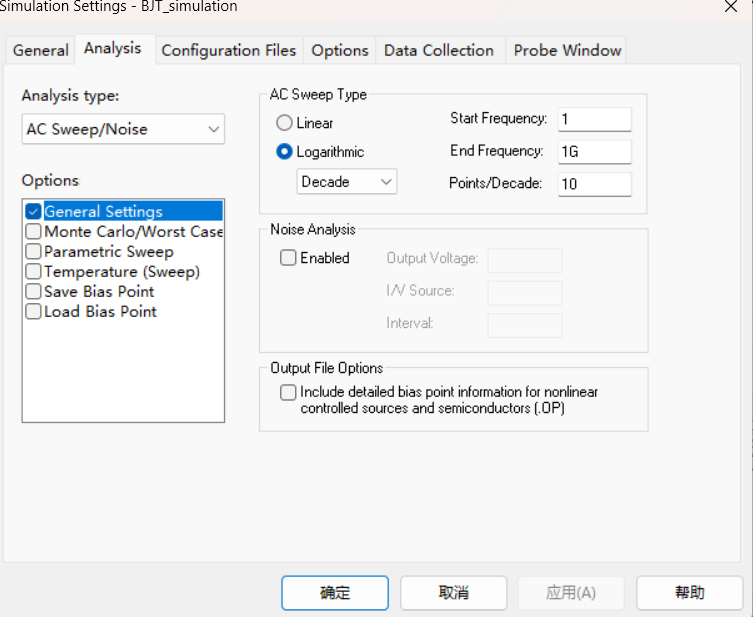
\includegraphics[width=\textwidth]{figure/Av_stifile_setting.png}
        \caption{交流分析参数设置}
        \label{fig:sub1}
    \end{subfigure}
    \hfill
    \begin{subfigure}[b]{0.32\textwidth}
        \centering
        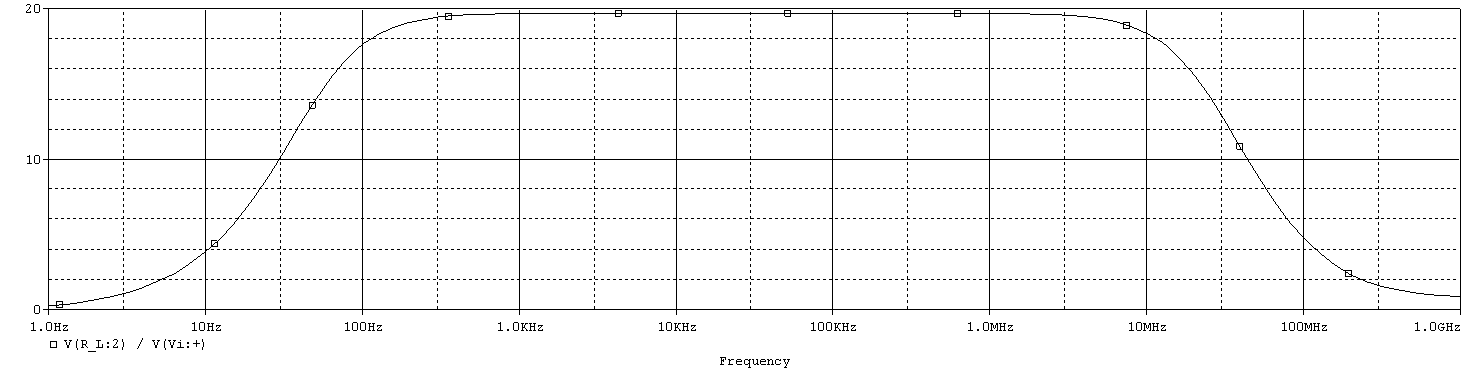
\includegraphics[width=\textwidth]{figure/Av_waveform.png}
        \caption{交流分析波形}
        \label{fig:sub2}
    \end{subfigure}
    \hfill
    \begin{subfigure}[b]{0.32\textwidth}
        \centering
        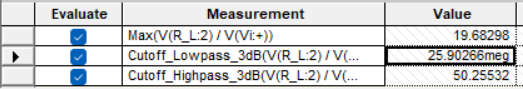
\includegraphics[width=\textwidth]{figure/Av_measure_result.png}
        \caption{交流分析测量结果}
        \label{fig:sub3}
    \end{subfigure}
    \caption{利用交流分析测量电压增益与截止频率}
    \label{fig:Av_f}
\end{figure}

(2)进行瞬态分析。运行后在 Probe 窗口中，添加 V(C2:2)和V(Vi:+)作输出，显示出时域波形，利用measure功能测得输出电压最大值为382.90304mV，
Vi最大值为19.99997mV，计算得$|Av|$=19.14518。
\begin{figure}[H]
    \centering
    \begin{subfigure}[b]{0.32\textwidth}
        \centering
        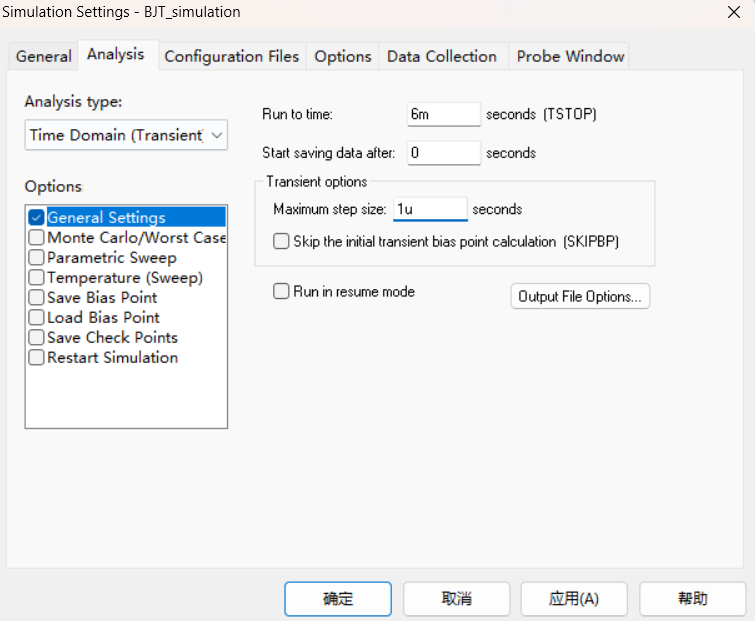
\includegraphics[width=\textwidth]{figure/Av_timefile_setting.png}
        \caption{瞬态分析参数设置}
        \label{fig:sub4}
    \end{subfigure}
    \hfill
    \begin{subfigure}[b]{0.32\textwidth}
        \centering
        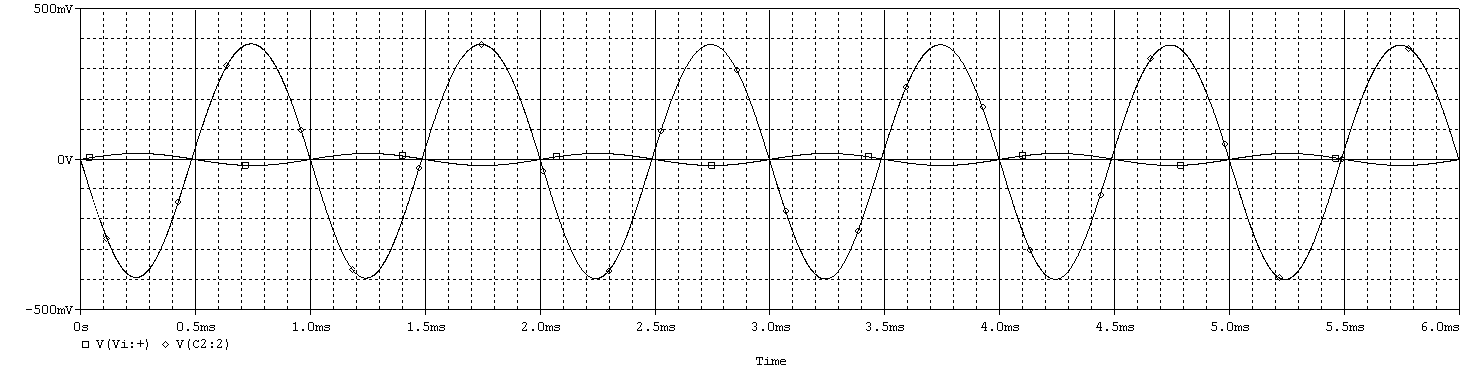
\includegraphics[width=\textwidth]{figure/Av_time_waveform.png}
        \caption{瞬态分析波形}
        \label{fig:sub5}    
    \end{subfigure}
    \hfill
    \begin{subfigure}[b]{0.32\textwidth}
        \centering
        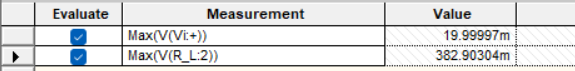
\includegraphics[width=\textwidth]{figure/Av_time_measure_result.png}
        \caption{瞬态分析测量结果}
        \label{fig:sub6}
    \end{subfigure}
    \caption{利用瞬态分析测量电压增益}
    \label{fig:Av_time_f}
\end{figure}
\subsubsection*{6.1.3 输入电阻与输出电阻}
测量输入电阻时采用交流分析，在 Probe 窗口中，执行 Trace/Add Trace 命令，选择
V（Vi:+）/I（C1）作输出量，显示出输入电阻的频率特性如图所示。启动标尺测出在 ƒ =1kHz
处的输入电阻$R_i \approx 6.4855k\Omega$
\begin{figure}[H]
    \centering
    \begin{subfigure}[b]{0.32\textwidth}
        \centering
        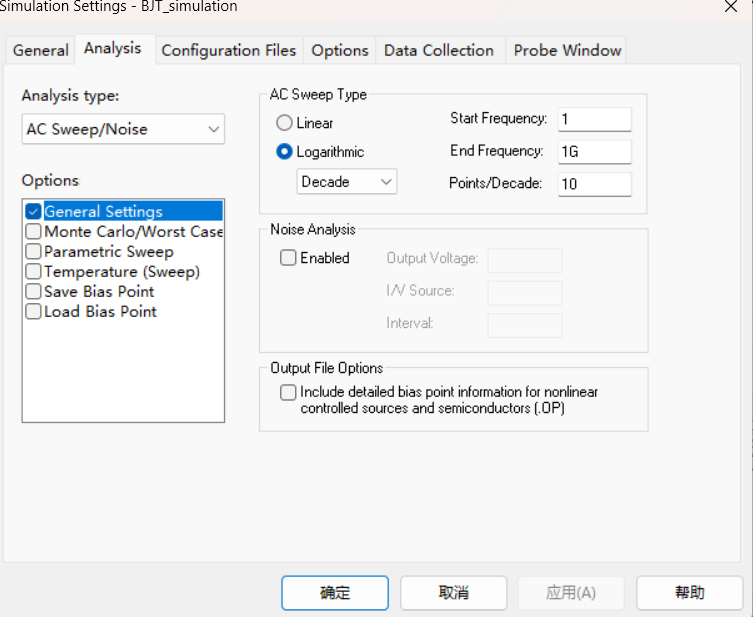
\includegraphics[width=\textwidth]{figure/Av_stifile_setting.png}
        \caption{输入电阻测量交流分析参数设置}
        \label{fig:Ri1}
    \end{subfigure}
    \hfill
    \begin{subfigure}[b]{0.32\textwidth}
        \centering
        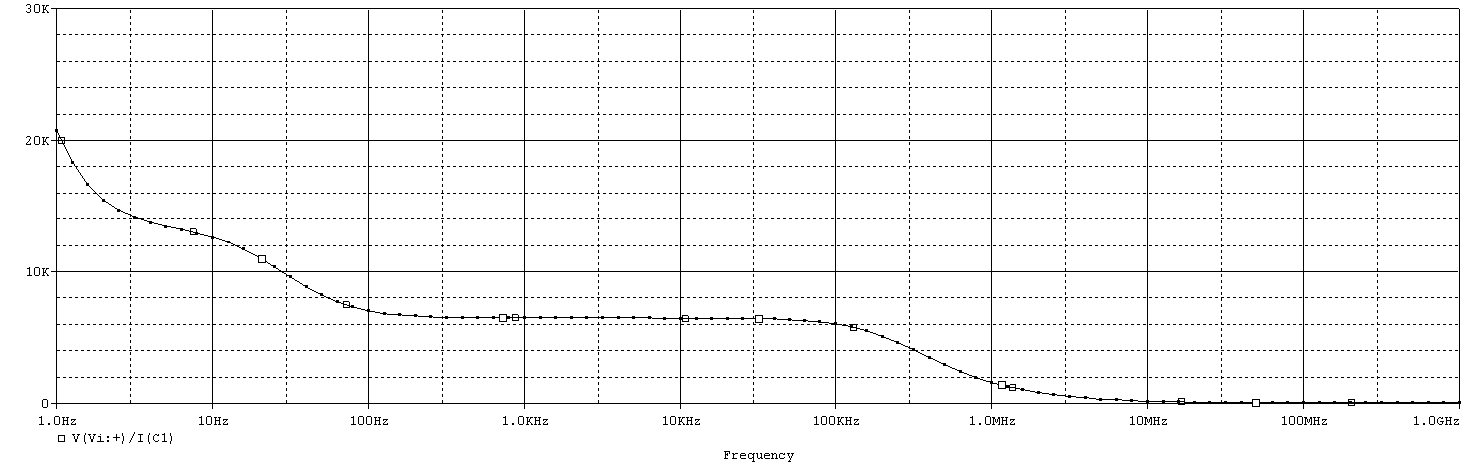
\includegraphics[width=\textwidth]{figure/Ri_waveform.png}
        \caption{输入电阻频率特性曲线}
        \label{fig:Ri2}
    \end{subfigure}
    \hfill
    \begin{subfigure}[b]{0.32\textwidth}
        \centering
        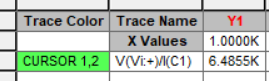
\includegraphics[width=\textwidth]{figure/Ri_measure_result.png}
        \caption{输入电阻仿真值}
        \label{fig:Ri3}
    \end{subfigure}
    \caption{}
    \label{fig:Ri}
\end{figure}

输出电阻：将电路的输入端短路，负载开路，在输出端加一信号源 Vo。进行交流分
析后，在 Probe 窗口中，执行 Trace/Add Trace 命令，选择 V(Vo:+)/I(Vo)作输出量，显
示出输出电阻的频率特性如图所示。启动标尺测出在 ƒ=1kHz 处的输出电阻 $R_o \approx 1.9820K \Omega$。
\begin{figure}[H]
    \centering
    \begin{subfigure}[b]{0.32\textwidth}
        \centering
        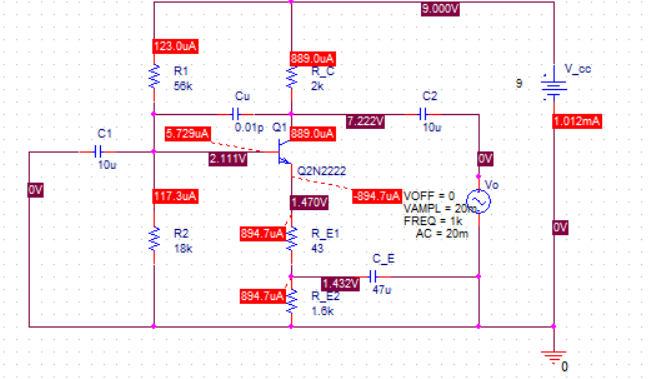
\includegraphics[width=\textwidth]{figure/Ro_circuit.png}
        \caption{输出电阻电路图}
        \label{fig:Ro1}
    \end{subfigure}
    \hfill
    \begin{subfigure}[b]{0.32\textwidth}
        \centering
        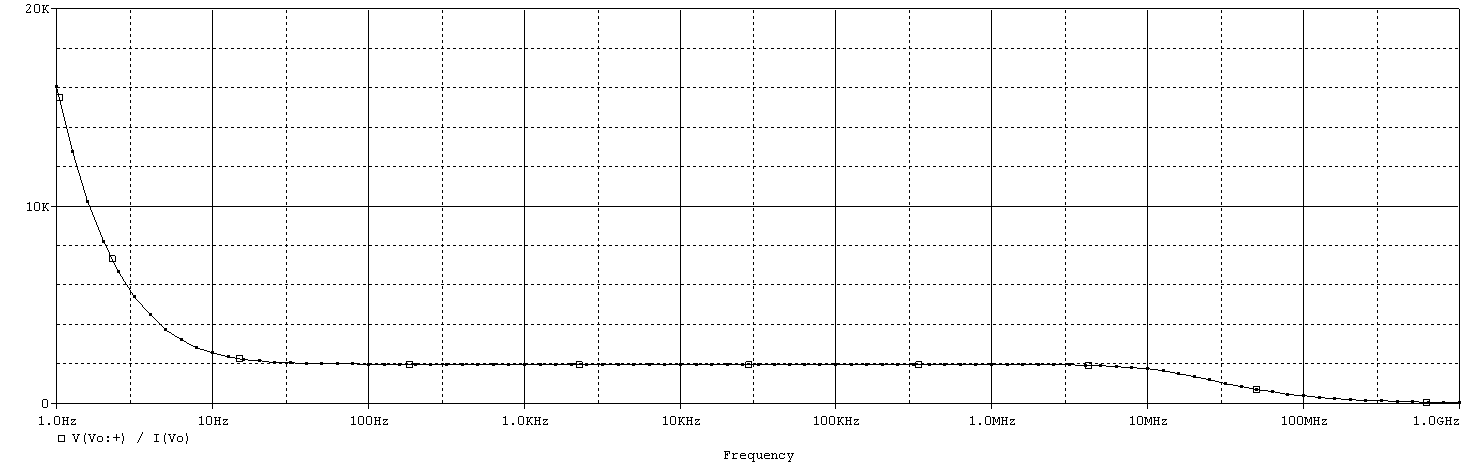
\includegraphics[width=\textwidth]{figure/Ro_waveform.png}
        \caption{输出电阻频率特性曲线}
        \label{fig:Ro2}
    \end{subfigure}
    \hfill
    \begin{subfigure}[b]{0.32\textwidth}
        \centering
        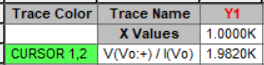
\includegraphics[width=\textwidth]{figure/Ro_measure_result.png}
        \caption{输出电阻仿真值}
        \label{fig:Ro3}
    \end{subfigure}
    \caption{}
    \label{fig:Ro}
\end{figure}
\subsubsection*{6.1.4 上限截止频率}
更改电路中的$C_u$值分别仿真。$C_u=0.01pF$时在测量电压增益时已得到$f_H = 25.90266MHz$。
$C_u=104pF$时如下图所示，测得$f_H' = 1.03274MHz$。
\begin{figure}[H]
    \centering
    \begin{subfigure}[b]{0.45\textwidth}
        \centering
        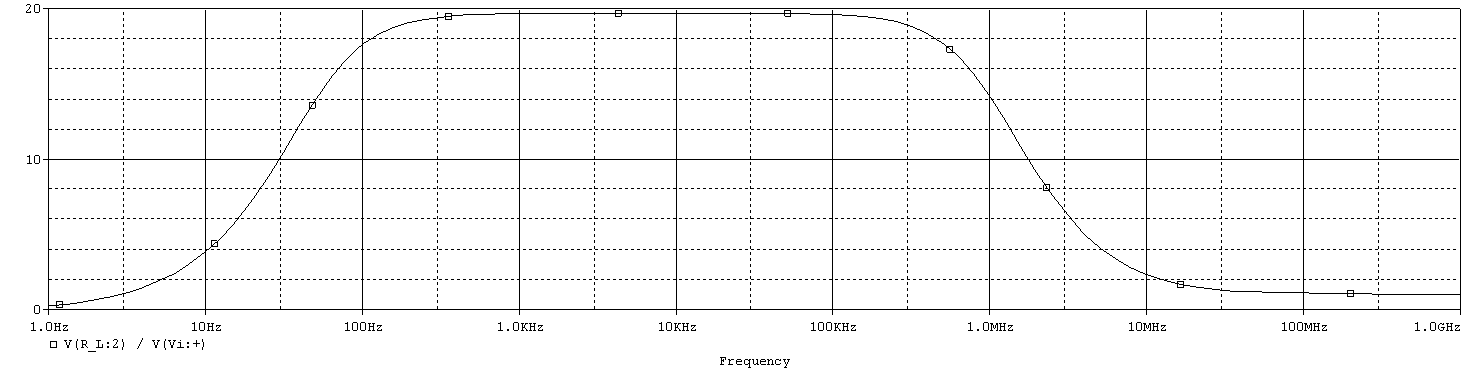
\includegraphics[width=\textwidth]{figure/fh104_waveform.png}
        \caption{$C_u=104pF$时电压增益频率特性曲线}
        \label{fig:fh_104_1}
    \end{subfigure}
    \hfill

    \begin{subfigure}[b]{0.45\textwidth}
        \centering
        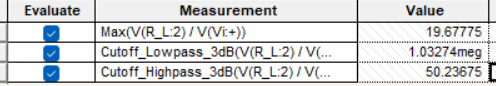
\includegraphics[width=\textwidth]{figure/fh104_measurement_result.png}
        \caption{$C_u=104pF$时上限频率仿真结果}
        \label{fig:fh_104_2}
    \end{subfigure}
    \hfill

    \caption{$C_u=104pF$时仿真结果}
    \label{fig:fh_104}
\end{figure}

$C_u=134pF$时如下图所示，测得$f_H(C_u) = 808.35313kHz$。
\begin{figure}[H]
    \centering
    \begin{subfigure}[b]{0.45\textwidth}
        \centering
        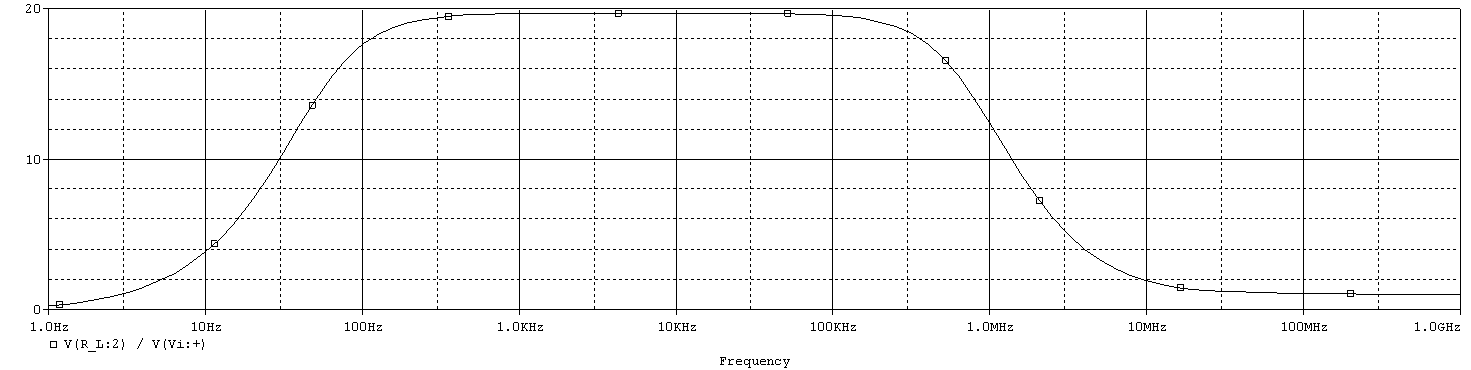
\includegraphics[width=\textwidth]{figure/fh134_waveform.png}
        \caption{$C_u=134pF$时电压增益频率特性曲线}
        \label{fig:fh_134_1}
    \end{subfigure}
    \hfill

    \begin{subfigure}[b]{0.45\textwidth}
        \centering
        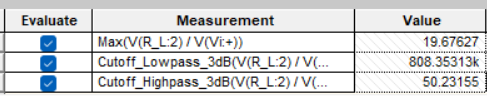
\includegraphics[width=\textwidth]{figure/fh134_measurement_result.png}
        \caption{$C_u=134pF$时上限频率仿真结果}
        \label{fig:fh_134_2}
    \end{subfigure}
    \hfill
    \caption{$C_u=134pF$时仿真结果}
    \label{fig:fh_134}
\end{figure}

汇总成表格如下：
\begin{table}[H]
    \centering
    \begin{tabular}{|c|c|}
    \hline
    $C_u$ (pF) & $f_H$ (MHz) \\
    \hline
    0.01 & 25.90 \\
    104 & 1.03 \\
    134 & 0.81 \\
    \hline
    \end{tabular}
    \caption{不同$C_u$值对应的上限截止频率}
    \label{tab:1.2}
\end{table}
\section*{七、数据分析与讨论}
\section*{7.1 静态工作点的调整与测量}
组装电路调节变阻器使$I_C$等于1mA设计值时测得静态工作点数据如下表所示：
\begin{table}[H]
\centering
\begin{tabular}{|c|c|c|c|}
\hline
 & 理论估算 & 测量 &仿真值 \\
\hline
$I_C(mA)$ &0.94 & 1.005 & 0.8947 \\
\hline
$V_{CE}(V)$ & 5.62 & 5.33 & 5.752\\
\hline
$V_{BE}(V)$ & 0.62 & 0.66 & 0.641\\
\hline
$V_B(V)$ & 2.14 & 2.34 & 2.111 \\
\hline
\end{tabular}
\caption{静态工作点数据对比表}
\end{table}
可以看到$V_{BE} \approx =0.6V$，发射结正向偏置，而$V_{CE}>V_{BE}-0.7$晶体管工作在放大区，符合预期。

\section*{7.2 电压增益的测量}
利用示波器的双踪显示观察输入输出波形，可以看到它们相位相反，符合共射放大电路的特性。通过测量输入输出电压幅值计算电压增益，
在不同测量条件下测量电压增益如下表格所示
\begin{table}[H]
\centering
\begin{tabular}{|l|c|c|c|c|c|c|}
\hline 
\multirow{2}{*}{测试条件} & \multicolumn{4}{c|}{实测值} & \multicolumn{1}{c|}{理论值}  & \multicolumn{1}{c|}{仿真值}\\
\cline{2-7} 
& $V_{\text{iP－P}}$ & $V_{\text{oP－P}}$ & $V_{\text{oP－Pmax}}$ & $\left|A_{\mathrm{V}}\right|$ & $\left|A_{\mathrm{V}}\right|$ & $\left|A_{\mathrm{V}}\right|$\\
\hline 
$R_{\mathrm{L}}=\infty$、有$\mathrm{C}_{\mathrm{E}}$ & 20.041 $\mathrm{mV}$ & $549.38 \mathrm{mV}$ & $3.05 \mathrm{V}$ & 27.41& 28.96 &27.32 \\
\hline 
$R_{\mathrm{L}}=\infty$、无$\mathrm{C}_{\mathrm{E}}$ & 20.048 $\mathrm{mV}$ & $23.750 \mathrm{mV}$ & $\times$ & 1.18 & 1.23 &1.19\\
\hline 
$R_{\mathrm{L}}$(5.1 $\mathrm{k}\Omega$)有$\mathrm{C}_{\mathrm{E}}$ & 19.964 $\mathrm{mV}$ & $391.09 \mathrm{mV}$& $\times$ & 19.59& 20.82 & 19.68\\
\hline 
\end{tabular}
\caption{电压增益测量数据表}
\end{table}
根据表格数据可以看到，负载电阻值的减小以及去掉电容$C_E$都会导致电压增益的降低，符合预期。
在$R_L$断路和$C_E$存在情况下逐步增大输入信号幅度，测得输出信号失真时的最大输出电压幅值为3.05V。
并且可以发现随着输入信号幅度增大，首先出现了截止失真，之后是饱和失真。失真波形如下所示：
\begin{figure}[H]
    \centering
    \begin{subfigure}[b]{0.32\textwidth}
        \centering
        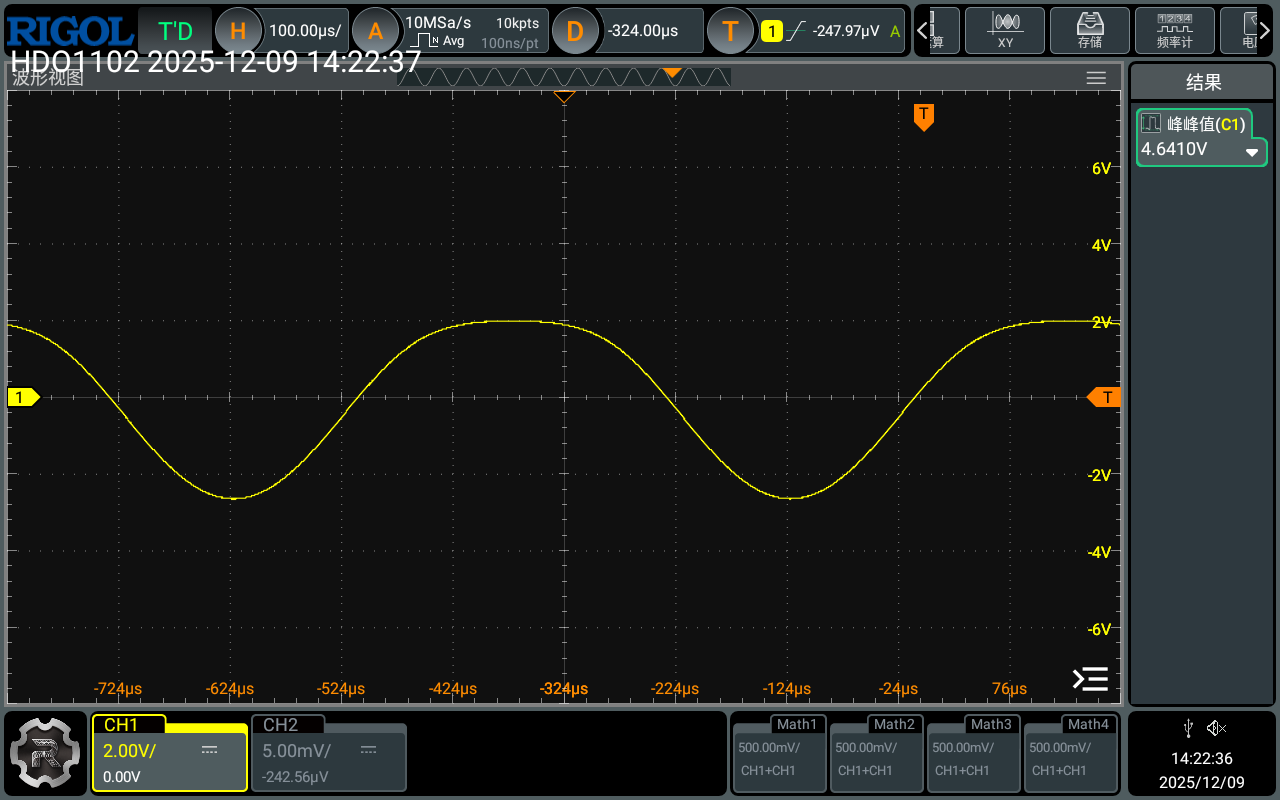
\includegraphics[width=\textwidth]{figure/cutoff_distort.png}
        \caption{截止失真波形}
        \label{fig:cutoff_distort}
    \end{subfigure}
    \hfill

    \begin{subfigure}[b]{0.32\textwidth}
        \centering
        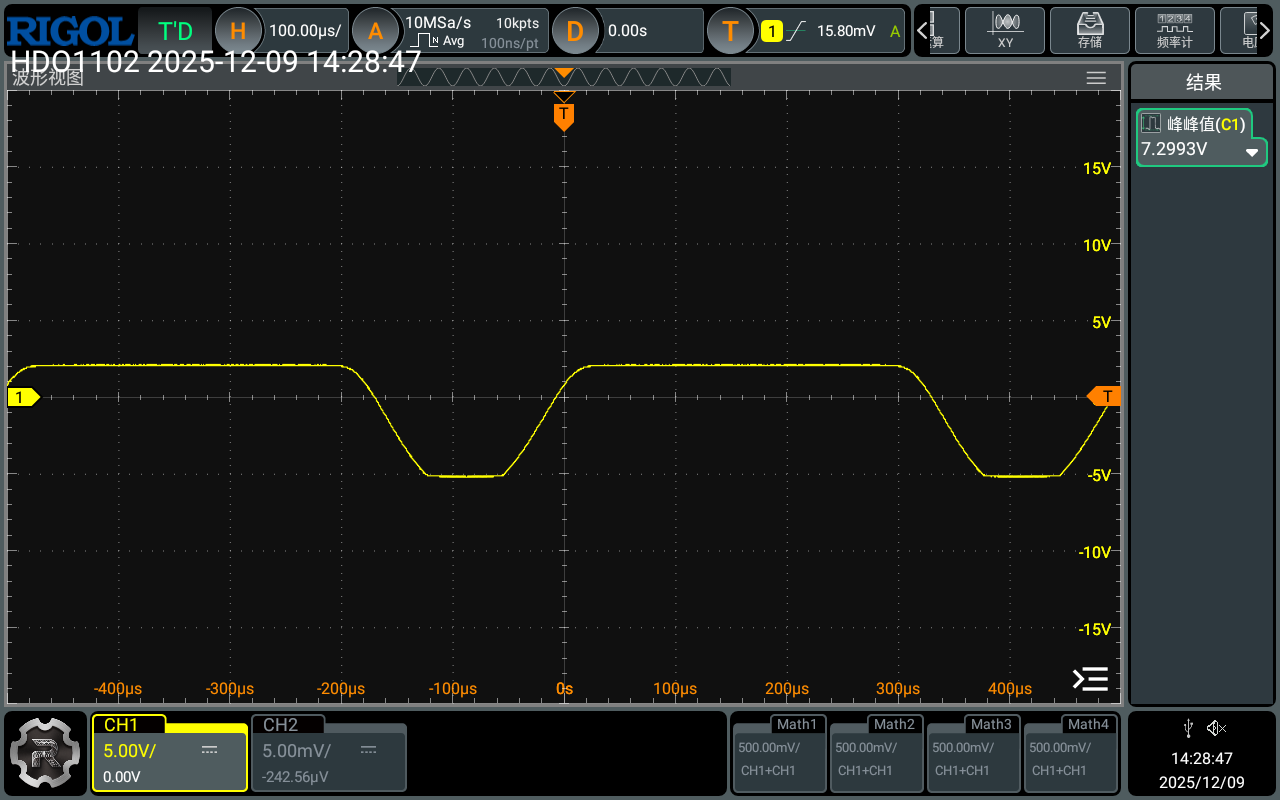
\includegraphics[width=\textwidth]{figure/sati_distort.png}
        \caption{饱和失真波形}
        \label{fig:sati_distort}
    \end{subfigure}
    \hfill

    \caption{失真波形图像}
    \label{fig:distort}
\end{figure}
\subsection*{7.3 输入电阻与输出电阻的测量}
在信号源与被测放大器之间串入一个与 $R_i$ 同一数量级（理论估算）的已知电阻 $R=5.1k \Omega$ ，在输出波形不失真的
情况下，分别测出 $v_s$ 和 $v_i$，则放大器的输入电阻为
\[R_i = R \frac{v_i}{v_s - v_i}\]
 \begin{table}[H]
\centering
\begin{tabular}{|c|c|c|c|c|c|}
\hline
$R_i$（理） & $R$ & $v_{\text{s}}$ & $v_{\text{i}}$ & $R_i$（实）&$R_i$(仿真) \\
\hline
 $5.21k \Omega$& $5.1 k \Omega$ & 981.0mV & 597.25 mV &  $7.93 k \Omega$ & $6.49k \Omega$\\
\hline
\end{tabular}
\caption{输入电阻测量数据表}
\end{table}
测量误差主要在于理论估算时$\beta$采用120，但是实际情况下$\beta$会有所偏差，导致计算的输入电阻与实际值存在差异。

输出波形不失真情况下，分别测出输出端空载时的输出电压 $v_o$、和接入负载 RL 后的输出电压 $v'_o$，则放大器的输出电阻为
\[R_o = R_L \frac{v_o - v'_o}{v'_o}\]
 \begin{table}[H]
\centering
\begin{tabular}{|c|c|c|c|c|c|}
\hline
$R_o$（理） & $R_L$ & $v_{\text{o}}$ & $v'_{\text{o}}$ & $R_o$（实）&$R_o$(仿真) \\
\hline
 $2k \Omega$& $5.1 k \Omega$ & 549.38 mV & 391.09 mV &  $2.06 k \Omega$ & $1.98k \Omega$\\
\hline
\end{tabular}
\caption{输出电阻测量数据表}
\end{table}
\section*{7.4 上限截止频率$f_H$和下线截止频率$f_L$的测量}
（1）在$I_C$为设计值1mA、$R_L=5.1\,\text{kΩ}$情况下，输入$v_i$（频率$2\,\text{kHz}$、幅度$10\,\text{mV}$的正弦信号），读出并记录输出电压峰-峰值$V_{Op-p}=392.56 mV$，计算$0.707V_{Op-p}=277.54 mV$。

（2）保持输入信号$v_i$的幅度不变，改变信号源的输出频率，当输出电压值达到$0.707V_{Op-p}$时，停止改变信号源频率，此时信号源对应的频率即为上限截止频率$f_H$或下限截止频率$f_L$。在无$C_u$情况下测出上限截止频率$f_H=1.0451\,\text{MHz}$，下限截止频率$f_L=62.578\,\text{Hz}$。

（3）插入电容$C_u=30\,\text{pF}$，测量并记录插入电容后的上限截止频率$f_{H(C_u)}=724.11 \text{kHz}$。
整理截止频率测量值与仿真值对比表格如下所示：
\begin{table}[H]
\footnotesize
\centering  
\begin{tabular}{|c|c|c|c|c|} 
\hline
 &  
$f_H$测量值&$f_H$仿真值& $f_L$测量值 & $f_L$仿真值 \\ 
\hline
无$C_u$& 1.0451\,\text{MHz} & 1.03\,\text{MHz}&62.578\,\text{Hz} &50.255 \,\text{Hz}\\
\hline  
有$C_u$&724.11 \text{kHz}&808.353\text{kHz}& $\times$ &$\times$\\
\hline
    \end{tabular}
    \caption{截止频率测量值仿真值对比表格} 
    \label{table:fH}
\end{table}


\section*{八、结论}
本次实验成功设计并实现了一个阻容耦合单级共射放大电路。
通过合理设置静态工作点（$I_C \approx 1mA$, $V_{CE} \approx 5.3V$），使晶体管工作在放大区。

实验测得电路主要性能指标为：电压增益 $|A_v| \approx 19.59$，输入电阻 $R_i \approx 7.93k\Omega$，输出电阻 $R_o \approx 2.06k\Omega$，下限截止频率 $f_L \approx 62.6Hz$，上限截止频率 $f_H \approx 1.05MHz$。
其中，电压增益与输入电阻均满足设计要求（$|A_v| > 15$，$R_i > 3k\Omega$），而下限截止频率略高于设计指标（$f_L < 50Hz$），原因可能在于旁路电容 $C_E$ 的取值仍有优化空间。通过引入分布电容 $C_u$ 验证了其对电路高频特性的影响，分布电容将导致上限截止频率显著降低。仿真结果与实测数据基本吻合，验证了理论分析的正确性和电路设计的可行性。

\section*{九、心得与体会}
通过本次实验，我深刻理解了晶体管共射放大电路的设计、调试与性能测试全过程。以下几点体会尤为深刻：

1.  理论与实践的结合：设计之初的理论计算和公式推导，为后续的元件参数选择提供了明确指导。然而，仿真和实测过程中，实际元件的参数离散性（如 $\beta$ 值）、测量误差以及分布参数（如 $C_u$）的存在，使得结果与理论值存在一定偏差。这让我认识到，理论模型是对现实的简化，在实际工程中必须通过仿真和调试来修正和完善设计。

2.  静态工作点的重要性：静态工作点是放大电路正常工作的基础。必须先建立合适、稳定的静态工作点，才能保证信号的有效放大。

3.  性能指标的权衡：在设计过程中，电压增益、输入电阻、通频带等指标往往相互制约。例如，为了提高增益，可以增大集电极电阻 $R_C$ 或减小 $R_{E1}$，但这可能影响静态工作点的稳定性或导致输出动态范围减小；为了提高输入电阻，可以增大基极偏置电阻，但这可能使静态工作点对晶体管参数的敏感度增加。这使我体会到电路设计是一个需要根据主要目标进行综合考量和折中的过程。

4.  仿真工具的辅助作用：在搭建实际电路前，利用Orcad等软件进行仿真，可以快速验证设计方案的可行性，预测电路性能，并能方便地研究参数变化对性能的影响（如 $C_u$ 对 $f_H$ 的影响），极大地提高了设计效率，降低了硬件调试的风险和成本。

5.  调试与测量技能的提升：在实际电路的焊接、调试和参数测量中，我掌握了示波器、信号发生器、万用表等仪器的规范使用方法，学习了如何通过观测波形判断电路工作状态，以及如何准确测量电压增益、输入/输出电阻和截止频率等关键指标。这些动手实践能力是理论学习无法替代的。示波器的使用了解了平均降噪、高频抑制、交流耦合等特殊功能模式。

总之，本次实验不仅巩固了模拟电子技术的基础知识，更锻炼了我综合运用理论分析、软件仿真和硬件调试来解决实际工程问题的能力。

\end{document}